\documentclass[acmsmall,screen,review,anonymous]{acmart}
\usepackage{amsmath}
\usepackage{booktabs}
\usepackage{tabularx}
\usepackage{listings}
\usepackage{algorithm}
\usepackage{algpseudocode}
\usepackage{tikz}
\usetikzlibrary{arrows.meta,positioning,fit,calc,backgrounds}
\definecolor{EvidenceBlue}{HTML}{315D80}
\definecolor{DecisionTeal}{HTML}{276B62}
\definecolor{RevisionAmber}{HTML}{98652D}
\definecolor{FigureInk}{HTML}{253342}
\definecolor{FigureRule}{HTML}{CAD2DA}
\algrenewcommand\algorithmicrequire{\textbf{Input:}}
\algrenewcommand\algorithmicensure{\textbf{Output:}}
\setcopyright{none}
\settopmatter{printacmref=false}
\acmDOI{}
\acmISBN{}
\acmConference[Research manuscript]{Research manuscript}{2026}{Anonymous draft}
\acmYear{2026}
\copyrightyear{2026}
\renewcommand\footnotetextcopyrightpermission[1]{}
\newcommand{\system}{ReachPatch}
\newcommand{\open}{\textsc{open}}
\newcommand{\blocked}{\textsc{blocked}}
\newcommand{\supported}{\textsc{supported}}
\newcommand{\refuted}{\textsc{refuted}}
\newcommand{\hash}{\operatorname{hash}}
\newcommand{\cost}{\operatorname{cost}}
\newcommand{\status}{\operatorname{status}}
\lstset{basicstyle=\ttfamily\small,columns=fullflexible,breaklines=true,showstringspaces=false,frame=single}
\title[Evidence-Driven Repair]{Repair Only When Evidence Demands It: Versioned Evidence Graphs for Cost-Aware Program Repair}
\author{Anonymous Author(s)}
\begin{abstract}
Repository-level repair agents repeatedly inspect source code, recover executable reproductions, and validate candidate patches. A shorter interaction can be cheaper, but it can also stop before collecting evidence needed to distinguish a repair from an overfitting patch. We investigate whether the need for further interaction can instead be expressed as an explicit, versioned evidence question. We present \system, a repair controller that maintains requirements, program locations, observations, candidate patches, and outstanding questions in one evidence graph. A deterministic scheduler selects repair, evidence recovery, or falsification actions from unresolved questions; recorded dependencies determine when a question must be reconsidered. Exact evidence identities suppress repeated actions without treating missing evidence as success. Our empirical audit identifies an important accounting sensitivity: a 20-issue retained-attempt pilot suggests a 29.3\% token reduction, whereas the completed 49-issue historical comparison records 21.45 versus 16.35 million tokens when archived attempts are included. Unequal retries and incomplete records preclude a causal interpretation of either contrast. We therefore separate this retrospective evidence from a prospective, blocked factorial study with durable request accounting and independent behavioral checks. The central research question is whether explicit evidence state can reduce the work requested of repair agents without abandoning necessary investigation; the current repository-level evidence does not yet establish that claim.
\end{abstract}
\begin{CCSXML}
<ccs2012><concept><concept_id>10011007.10011074.10011099</concept_id><concept_desc>Software and its engineering~Software verification and validation</concept_desc><concept_significance>500</concept_significance></concept><concept><concept_id>10011007.10011074.10011092</concept_id><concept_desc>Software and its engineering~Software evolution</concept_desc><concept_significance>300</concept_significance></concept></ccs2012>
\end{CCSXML}
\ccsdesc[500]{Software and its engineering~Software verification and validation}
\ccsdesc[300]{Software and its engineering~Software evolution}
\keywords{automated program repair, evidence reuse, agent efficiency, demand-driven validation}
\begin{document}
\maketitle

\section{Introduction}
The cost of a repair agent is not determined solely by the size of its final patch. The agent may repeatedly inspect the same implementation, reconstruct a reproduction that already exists, or reconsider an observation whose relevant context has not changed. Each interaction also carries some of the preceding trajectory into another model request. Recent work demonstrates that this accumulated context contains removable waste: AgentDiet reduces trajectories during execution while accounting for the cost of the reduction model itself~\cite{xiao2026agentdiet}. Other work improves the granularity of debugging interactions~\cite{xiang2026adi} or assigns different editing subtasks to different-sized models~\cite{wang2026cascade}. These findings make efficiency a substantive program-repair research problem, rather than merely an implementation concern.

An additional question arises \emph{before} an interaction is issued: what unresolved fact would justify doing this work again? An agent may have already read a source span, yet a subsequent patch can make that read stale. A reproduction may execute successfully, yet establish nothing about the behavior requested in the issue. Conversely, the relevant evidence may be unchanged, making another recovery round unnecessary. Neither a fixed repair--test alternation nor indiscriminate memoization distinguishes these situations. The first repeats work; the second risks retaining conclusions after their supporting evidence changes.

We study this distinction through \emph{versioned evidence questions}. A question identifies an unresolved claim about a candidate patch, the evidence on which its answer depends, and the conditions under which that answer must be revisited. For example, ``does the reported operation satisfy the stated boundary behavior?'' differs from ``can the reproduction import the intended module?'' The former may justify a repair or a counterexample; the latter justifies resolving an execution prerequisite. Repeating either action without a change in its question or evidence is a candidate for suppression. Importantly, an unanswered or blocked question is not a passing check.

\system{} stores these questions in the same graph as source locations, observations, validation obligations, and patch checkpoints. This is an operational evidence graph, not a separate search tree augmented with graph-shaped prompt context. The controller queries the graph to select an action, records what the action established, and revisits questions when their recorded versions change. Repair proposes a code change; falsification challenges a specific outstanding claim. Deterministic discovery and execution precede model-based recovery where the necessary operation is already known. The model remains responsible for constructing repairs and probes that cannot be obtained by those deterministic steps.

Our intended objective is lower end-to-end cost subject to retained repair effectiveness. It is not more candidate patches, more graph nodes, or a lower token count obtained by refusing difficult issues. It is also not a claim that the repair and falsification roles reach a game-theoretic equilibrium: the implemented scheduler uses deterministic evidence priorities, not a learned utility function or an equilibrium solver.

This manuscript makes three bounded contributions. First, it formulates repair interaction as scheduling versioned evidence questions and identifies the conditions under which reuse is admissible. Second, it describes a concrete controller that combines question-driven scheduling, exact reuse, and explicit stopping states within one graph. Third, it audits the difference between retained-attempt savings and all-attempt expenditure, and operationalizes a controlled study to distinguish scheduling benefits from premature stopping. The historical evidence does not establish an effectiveness--cost advantage: lower retained-attempt cost alone cannot distinguish avoided work from abandoned or retried work.

\section{Motivation and Research Objective}
\subsection{Repeated work is state-dependent}
Consider the illustrative implementation in Listing~\ref{lst:example}. The issue requires a missing limit to select a default, while an explicit zero must remain zero. A nearby public test also requires negative limits to be rejected. The example is constructed to explain the mechanism; it is not presented as a measured benchmark outcome.

\begin{lstlisting}[language=Python,caption={Illustrative boundary bug with distinct target and preservation questions.},label=lst:example]
def normalize_limit(limit):
    if not limit:
        return 10
    if limit < 0:
        raise ValueError("negative limit")
    return limit
\end{lstlisting}

The initial read identifies the truthiness predicate. A reproduction of \texttt{normalize\_limit(0)} returns 10 and supplies a stable target failure when repeated. If the agent asks for the identical source range again before editing it, the recorded source hash can identify an exact read reuse opportunity. If it changes the predicate to \texttt{limit is None}, however, the earlier source observation is stale. The target question must be re-evaluated for the new patch.

A repair that also deletes the negative-limit guard creates a different unresolved question: has the patch preserved the public rejection behavior? Repeating target recovery does not answer it. A targeted negative-input check does. If that check fails, the next repair should preserve the zero-input success while restoring rejection, rather than discard both changes. If a generated input has no grounded expected behavior, executing it may still reveal a path or exception, but its result cannot be promoted to a trusted pass or regression.

This example separates three identities that are often conflated: the identity of a \emph{request}, the identity of its \emph{evidence context}, and the identity of the \emph{claim} being investigated. Identical commands can be useful after an edit. Different commands can redundantly investigate the same unresolved claim. Our implementation suppresses only supported exact identities; it does not solve general semantic equivalence between commands or hypotheses.

\subsection{Objective and scope}
For a fixed issue distribution, let $Y_i^\pi$ indicate whether the single patch selected by policy $\pi$ resolves issue $i$ under held-out evaluation. Let $C_i^\pi$ include all model requests and retries needed to produce that patch. The intended objective is
\begin{equation}
 \min_\pi\;\mathbb{E}[C_i^\pi]
 \quad\text{subject to}\quad
 \mathbb{E}[Y_i^\pi-Y_i^{\pi_0}]\geq-\delta,
 \label{eq:objective}
\end{equation}
where $\pi_0$ is a matched baseline and $\delta$ is a non-inferiority margin fixed before evaluation. This expression defines an experimental objective, not an optimization problem solved by our controller. Tokens, billed cost, model calls, and elapsed time are reported separately: provider caching and concurrency prevent them from being interchangeable.

The controller observes the issue description, the base repository, accessible public tests, and its own executions, following the repository-level issue setting of SWE-bench~\cite{jimenez2024swebench}. It does not observe the benchmark's hidden tests or reference repair during generation. It returns one full base-to-selected-patch diff. An internally certified patch satisfies the available executable obligations; it is not a proof that the issue is fully repaired. Accordingly, internal certification and externally measured Resolved@1 are different outcomes throughout this paper.

\section{Versioned Evidence as Repair State}
\subsection{One graph, multiple decision views}
At step $t$, the controller maintains a typed graph $G_t=(V_t,E_t)$. The graph connects a candidate patch to the claims it must satisfy and to the observations that bear on those claims. Its essential relation is not simply that two entities are adjacent, but that a decision depends on a particular piece of evidence. For example, a checkpoint $p$ requires validation of a question $q$; $q$ derives from requirement $r$ and source evidence $d$; and an execution observation $o$ supports or refutes the claim in $q$. These links preserve the path from a repair decision back to its justification.

Two graph views are central to this dependency semantics. Let $\mathcal{Q}(G,p)$ denote the questions associated with checkpoint $p$, and let $\mathcal{D}(G,q)$ denote the dependencies recorded for question $q$. The scheduler operates on the open-question frontier
\begin{equation}
 \mathcal{F}_Q(G)=\{(p,q)\mid p\in\mathcal{P}_{\mathrm{open}}(G),\;
 q\in\mathcal{Q}(G,p),\;\status_G(q)=\open\},
 \label{eq:question-frontier}
\end{equation}
where $\mathcal{P}_{\mathrm{open}}(G)$ contains checkpoints still eligible for investigation. The dependency view determines the recorded state used to version each question. Together, these views let the controller ask both \emph{what remains unresolved?} and \emph{has the evidence for an earlier answer changed?} Figure~\ref{fig:loop} illustrates the connection. Neither view creates a second graph.

Program and execution relations refine the evidence attached to these questions. Static calls and approximate def--use identify possible dependencies; observed calls, branch outcomes, and failure locations record what an execution actually reached. The distinction prevents a possible path from becoming evidence that a requirement was exercised. Modification and localization links associate a hypothesis with the source it proposes to change, while closure and regression links retain the outcomes of evaluating that change.

Program evidence is seeded before initial patch generation from issue symbols, source hints, public checks, and bounded local source analysis. Executions then add observations and dynamic paths. The implementation limits source exploration by files, symbols, edges, depth, and time; budget boundaries remain explicit frontiers. A missing edge at the graph budget must not silently remove an executable validation obligation: the validation view also examines applicable obligation nodes. The graph therefore records both what is known and where exploration stopped.

Each checkpoint contains the complete diff from the base revision and its own executable evidence. A hypothesis denotes an intended mechanism, a parent checkpoint, and supporting locations. If two hypotheses produce the exact same patch hash and full diff, the later hypothesis can point to the existing checkpoint through a transposition relation. This creates a search \emph{graph}, rather than a tree whose identical states necessarily remain separate. Patch equality does not by itself establish environment equivalence or permit reusing an execution result.

\subsection{Questions and versions}
A question is represented conceptually as
\begin{equation}
 q=\langle k,c,p,R,D,E,s,b,\nu\rangle,
\end{equation}
where $k$ is the action-related kind, $c$ the claim, $p$ the checkpoint, $R$ the requirements, $D$ the dependencies, $E$ the supporting evidence, $s$ the status, $b$ a blocking reason, and $\nu$ the evidence version. Questions and action records are obligation subtypes in the same graph, not an additional graph structure.

The implementation forms a stable question identifier from the checkpoint, kind, claim, requirement identifiers, and dependency identifiers. Its version hashes the patch identity, explicitly supplied relevant state, and the recorded revision and status of existing dependency and evidence nodes:
\begin{equation}
 \nu(q,G)=\hash\!\left(h_p,z_q,
       [(d,\operatorname{rev}_G(d),\status_G(d))]_{d\in D\cup E}\right).
 \label{eq:version}
\end{equation}
Here $z_q$ can contain semantic execution signatures, mechanical blockers, or a validation audit. This is a conservative recorded-state identity, not a minimal semantic dependence analysis. Because the full patch identity is included, unrelated edits can reopen a question. Conversely, unrecorded external state cannot be detected by this version alone.

A newly created question is \open. An observation may support or refute its claim, or establish a blocking reason. A replaced question can be superseded. When the recorded version changes, an existing question becomes open again. \blocked{} means that the controller lacks an admissible next step for that question under the current evidence and budget. It does not imply that its claim is true.

\subsection{Authority is distinct from observation}
An executable probe specifies its input, entrypoint, environment, observation adapter, and comparator. Executing the probe provides an observation; it does not create an oracle. Certification requires an expected behavior grounded in accepted public evidence, such as a public test or an explicit issue requirement with a traceable source binding. A model may propose a comparator, but cannot grant it authority by asserting that the comparator is correct.

This distinction matters for boundary challenges. A changed truthiness predicate suggests trying missing, empty, and nonempty values. It does not establish that all three inputs should be accepted. A challenge with an input but no grounded expectation remains exploratory. Its execution may refine localization or reveal a blocker, while leaving the corresponding specification question unresolved. Similarly, syntax checks and imports are mechanical prerequisites, not substitutes for executing the required target behavior.

\section{Demand-Driven Repair and Falsification}
\subsection{From evidence gaps to actions}
The controller first attempts deterministic requirement extraction, source discovery, and available reproduction construction. It then generates an initial patch with bounded source context. After that patch, evidence recovery is reconsidered when executable target evidence or validation coverage is missing. This ordering avoids paying a model to orchestrate execution steps that already have a known implementation, while retaining model-based recovery for unresolved entrypoints or probe constructions.

The scheduler derives eligible actions from every open checkpoint in the graph. Its current priority order places mechanical repair first; missing validation and locked-success regression next; final review and eligible exploratory probes next; missing evidence recovery next; other stable failures next; and bounded graph expansion last. Preconditions resolve overlaps: a checkpoint without observations first requires validation, and an exhausted repair frontier may instead request expansion. This is a concrete heuristic policy, not an estimate of expected information gain.

Within a priority class, selection is lexicographic. For action $a$ at checkpoint $p$, the ordering key is
\begin{equation}
 \rho_G(a)=\bigl(\pi(a),-\widehat{\mathbf{s}}_G(p,a),
 -|O_a|,v_G(p),\widehat{\tau}_G(a),\operatorname{id}(a)\bigr),
 \label{eq:action-order}
\end{equation}
where $\pi$ is the priority class, $\widehat{\mathbf{s}}$ the executable-evidence score vector, $O_a$ the associated obligations, $v$ the visit count, and $\widehat{\tau}$ the estimated duration. The vector is negated componentwise so that stronger evidence sorts first. For expansion actions, the score may include best-descendant potential; validation and certification use the checkpoint's own evidence. Duration is the median of recorded durations for the action kind when available, with a validation-specific estimate from recorded runs as a fallback; unknown cost sorts last. No model call is used to compute this ordering.

\begin{figure}[t]
\centering
% Native vector artwork. All three panels are projections of one mutable graph.
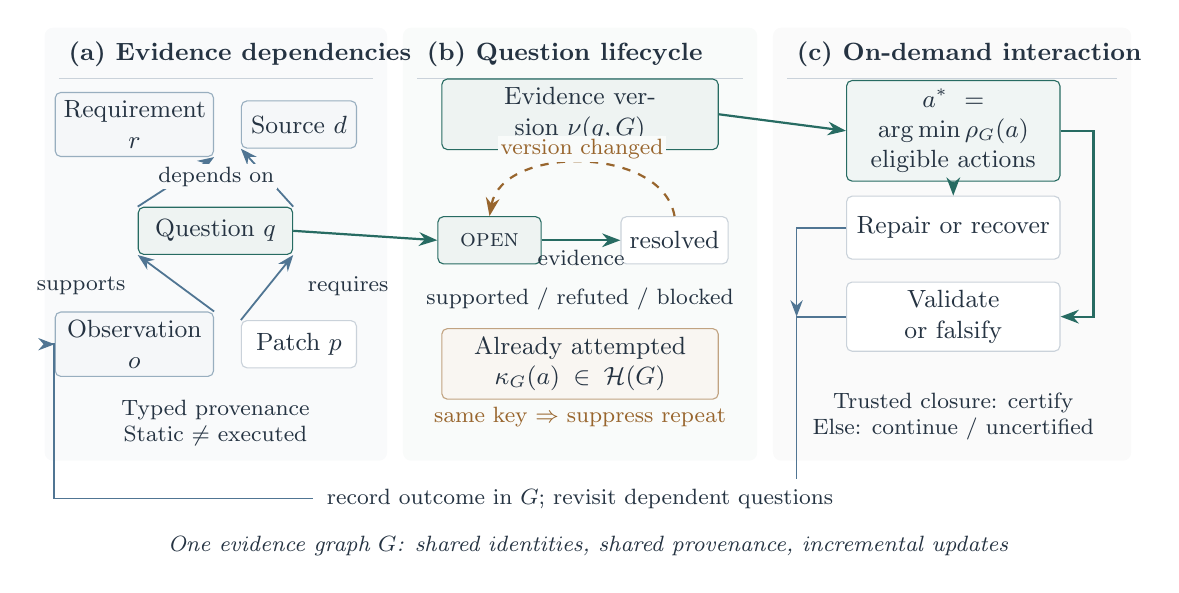
\begin{tikzpicture}[
  x=1cm,y=1cm,>=Stealth,
  every node/.style={font=\small,text=FigureInk},
  heading/.style={font=\small\bfseries,anchor=west},
  entity/.style={draw=FigureRule,fill=white,rounded corners=2pt,
    minimum height=6mm,inner sep=3pt,align=center},
  evidence/.style={entity,draw=EvidenceBlue!50,fill=EvidenceBlue!5},
  question/.style={entity,draw=DecisionTeal,fill=DecisionTeal!8},
  edge/.style={->,draw=EvidenceBlue!85,line width=.65pt},
  control/.style={->,draw=DecisionTeal,line width=.8pt},
  revision/.style={->,draw=RevisionAmber,dashed,line width=.8pt},
  detail/.style={font=\footnotesize,align=center},
  action/.style={entity,text width=2.5cm,minimum height=8mm}
]
% Panel geometry remains fixed at the ACM single-column width.
\fill[EvidenceBlue!3,rounded corners=3pt] (0,0) rectangle (4.35,5.5);
\fill[DecisionTeal!3,rounded corners=3pt] (4.55,0) rectangle (9.05,5.5);
\fill[black!2,rounded corners=3pt] (9.25,0) rectangle (13.8,5.5);
\node[heading] at (.18,5.16) {(a) Evidence dependencies};
\node[heading] at (4.73,5.16) {(b) Question lifecycle};
\node[heading] at (9.43,5.16) {(c) On-demand interaction};
\draw[FigureRule] (.18,4.86)--(4.17,4.86);
\draw[FigureRule] (4.73,4.86)--(8.87,4.86);
\draw[FigureRule] (9.43,4.86)--(13.62,4.86);
% A small real dependency graph, not a module inventory.
\node[evidence,text width=1.8cm] (req) at (1.14,4.27) {Requirement\\$r$};
\node[evidence,text width=1.25cm] (src) at (3.23,4.27) {Source $d$};
\node[question,text width=1.75cm] (claim) at (2.17,2.92) {Question $q$};
\node[evidence,text width=1.8cm] (obs) at (1.14,1.48) {Observation\\$o$};
\node[entity,text width=1.25cm] (patch) at (3.23,1.48) {Patch $p$};
\draw[edge] (claim.north west)--(req.south east);
\draw[edge] (claim.north east)--(src.south west);
\node[detail,fill=EvidenceBlue!3,inner sep=1pt] at (2.18,3.61) {depends on};
\draw[edge] (obs.north east)--(claim.south west);
\draw[edge] (patch.north west)--(claim.south east);
\node[detail,anchor=east] at (1.15,2.22) {supports};
\node[detail,anchor=west] at (3.22,2.22) {requires};
\node[detail] at (2.17,.48)
  {Typed provenance\\Static $\neq$ executed};
% Evidence-version lifecycle. Each outcome is explicitly named.
\node[question,text width=3.3cm] (version) at (6.8,4.4)
  {Evidence version $\nu(q,G)$};
\node[question,text width=1.1cm] (openq) at (5.65,2.8) {\textsc{open}};
\node[entity,text width=1.15cm] (answered) at (8.0,2.8) {resolved};
\draw[control] (openq)--node[below,detail]{evidence}(answered);
\draw[revision] (answered.north) to[out=100,in=80]
  node[above,detail,text=RevisionAmber,fill=DecisionTeal!3,inner sep=1pt]
  {version changed} (openq.north);
\node[detail] at (6.8,2.05)
  {supported / refuted / blocked};
\node[entity,draw=RevisionAmber!60,fill=RevisionAmber!6,
  text width=3.3cm] (reuse) at (6.8,1.23)
  {Already attempted\\$\kappa_G(a)\in\mathcal H(G)$};
\node[detail,text=RevisionAmber] at (6.8,.56)
  {same key $\Rightarrow$ suppress repeat};
% Actions are alternatives selected from a global frontier, not fixed stages.
\node[action,draw=DecisionTeal,fill=DecisionTeal!7] (select) at (11.54,4.19)
  {$a^*=\arg\min\rho_G(a)$\\eligible actions};
\node[action] (repair) at (11.54,2.96) {Repair or recover};
\node[action] (test) at (11.54,1.83) {Validate or falsify};
\node[detail] at (11.54,.56)
  {Trusted closure: certify\\Else: continue / uncertified};
\draw[control] (select.south)--(repair.north);
\draw[control] (select.east)--(13.32,4.19)--(13.32,1.83)--(test.east);
% Sparse cross-panel links avoid passing through labels or evidence nodes.
\draw[control] (claim.east)--(openq.west);
\draw[control] (version.east)--(select.west);
\draw[edge] (test.west)--(9.55,1.83)--(9.55,-.48)--(.12,-.48)--(.12,1.48)--(obs.west);
\draw[edge] (repair.west)--(9.55,2.96)--(9.55,1.83);
\node[detail,fill=white,inner xsep=5pt] at (6.8,-.48)
  {record outcome in $G$; revisit dependent questions};
\node[font=\footnotesize\itshape,text=FigureInk] at (6.9,-1.08)
  {One evidence graph $G$: shared identities, shared provenance, incremental updates};
\end{tikzpicture}

\caption{Evidence-dependent interaction in \system. (a) A question links a checkpoint to its requirement, source, and execution evidence. (b) Recorded dependency changes reopen the question; an unchanged attempted action is suppressed under its reuse key. (c) The selected action returns evidence to the same graph. Certification requires trusted executable closure; blocked or exhausted evidence leads to an uncertified output, not success. Solid arrows denote evidence or control flow; the dashed feedback denotes version invalidation. The three panels are views of one state, not separate graph objects.}
\Description{Three aligned panels show an evidence graph, a versioned question lifecycle, and demand-driven actions. Requirement, source and observation nodes connect to a question and checkpoint. An open question yields an action, while an already attempted unchanged key is suppressed. Execution feeds new evidence back to the graph; changed versions reopen questions. Certification and uncertified termination are distinct.}
\label{fig:loop}
\end{figure}

Algorithm~\ref{alg:scheduler} specifies the outer control policy. $\mathcal{A}(G)$ contains eligible actions derived from the open-question frontier, subject to execution and search preconditions. An action key $\kappa_G(a)$ combines its question, kind, and relevant evidence version; $\mathcal{H}(G)$ is the set of recorded attempted keys. Both are graph views, not external search state. \textsc{Dispatch} performs the selected operation with the remaining budget and returns its outcome and measured usage. \textsc{Integrate} records observations, patch provenance, question outcomes, and exhausted actions, including blocked executions. The production paths for recovery, validation, and generation implement this abstraction separately; it does not imply a universal interception gate for every internal model tool call.

\begin{algorithm}[t]
\caption{Evidence-dependent repair and falsification}
\label{alg:scheduler}
\begin{algorithmic}[1]
\Require Base repository $R_0$, issue $I$, public evidence $E_0$, budget $B$
\Ensure Full base-to-selected diff $\Delta^*$, decision $z$, evidence graph $G$
\State $G \gets \Call{Seed}{R_0,I,E_0}$
\State $(G,p_0,B) \gets \Call{Bootstrap}{G,R_0,I,B}$
\Comment{Recovery, initial patch, and evidence gaps}
\While{$\Call{WithinBudget}{B}$}
  \ForAll{$q\in\Call{Questions}{G}$}
    \State $\nu' \gets \nu(q,G)$ \Comment{Equation~\eqref{eq:version}}
    \If{$\nu'\neq q.\nu$}
      \State $(q.s,q.\nu)\gets(\open,\nu')$
    \EndIf
  \EndFor
  \State $\mathcal{C}\gets\{p\in\Call{Evaluated}{G}\mid\Call{Certified}{p,G}\}$
  \If{$\mathcal{C}\neq\varnothing$}
    \State \Return $(\Delta(\Call{Select}{\mathcal{C},G}),\textsc{certified},G)$
  \EndIf
  \State $\mathcal{A}\gets\Call{EligibleActions}{G,B}$
  \Comment{Questions and execution prerequisites}
  \ForAll{$a\in\mathcal{A}$ such that $\Call{ReuseEnabled}{a,G}$}
    \If{$\kappa_G(a)\in\mathcal{H}(G)$}
      \State $G\gets\Call{RecordSuppression}{G,a}$; $\mathcal{A}\gets\mathcal{A}\setminus\{a\}$
    \EndIf
  \EndFor
  \If{$\mathcal{A}=\varnothing$}
    \State \textbf{break} \Comment{No admissible action; not evidence of success}
  \EndIf
  \State $a^*\gets\arg\min_{a\in\mathcal{A}}\rho_G(a)$ \Comment{Equation~\eqref{eq:action-order}}
  \State $G\gets\Call{RecordAttempt}{G,a^*,\kappa_G(a^*)}$
  \State $(y,u)\gets\Call{Dispatch}{a^*,R_0,G,B}$
  \Comment{Repair, recover, validate, probe, expand, or review}
  \State $G\gets\Call{Integrate}{G,a^*,y}$; $B\gets\Call{Debit}{B,u}$
\EndWhile
\State $p^*\gets\Call{BestAdmissibleEvaluated}{G}$
\State $z\gets\Call{FinalStatus}{p^*,G,B}$
\Comment{Certified only if executable closure holds}
\State \Return $(\Delta(p^*),z,G)$
\end{algorithmic}
\end{algorithm}

\subsection{Repair and targeted falsification}
For a stable failure, localization ranks causal cuts using failure frames, executed paths, relevant value flow, and changed source. A cut provides real source spans and observations, rather than only graph identifiers. The repair request identifies the parent patch, the failed command, expected and actual observations, the proposed mechanism, and successes that must be preserved. Each candidate starts from its specified parent; its output is a complete base-to-child diff.

Falsification addresses a remaining claim about that candidate. The graph connects changed predicates and value-flow paths to boundary input recipes and affected checkpoints. Only executable, authority-grounded challenges can strengthen or refute certification. Exploratory probes are separately bounded. This makes the falsification role operationally different from a second model producing an unrestricted critique: a critique without an executable or evidence-recovery consequence does not establish a counterexample.

Rejected candidates remain in the graph with their failure evidence. The workspace can be restored to the recorded parent, and global selection can choose another checkpoint. A candidate that progresses on the target but regresses on a preservation obligation remains useful as a repair state, with passing target obligations locked. Retaining such a state supports repair of the regression without treating the candidate as final. Exact patch transpositions preserve alternative provenance without claiming a new distinct patch.

\subsection{Three different forms of reuse}
\paragraph{Action suppression.}
An action identity contains its question identity, kind, and evidence version. With suppression enabled, admission records an in-flight action before execution and rejects another attempt with the same stable identity. Execution then distinguishes completed work, retryable failure, and other failure. A transport error, timeout, or malformed JSON response permits one additional admission under the same identity, for at most two attempts in total; completed actions and exhausted retries remain suppressed. Changed evidence creates a new version rather than reusing the old result. This bounded policy neither guarantees exactly-once execution nor treats a failed interaction as evidence that the underlying question is resolved. Its false-suppression risk is an empirical safety question.

\paragraph{Evidence and context reuse.}
Source observations are keyed by path, content hash, and line range. A changed content hash marks previous source evidence stale. This identifies representational reuse; it need not eliminate physical file I/O when the caller has already computed the result. Within a model request, exact duplicate tool payloads can be replaced by shorter references only when the first full payload remains in that same request. Unique payloads and message envelopes remain intact. A later API call is not presumed to remember a previous request. Byte elision is recorded separately from provider-reported tokens.

\paragraph{Validation reuse.}
Execution caching is opt-in. A check must attest that it is isolated and deterministic, has no external state, and identifies its environment. Its key additionally includes clean and working tree hashes, the full check specification, an inherited-environment hash, execution backend metadata, adapter hashes, and the stability-run count. Only stable pass or fail results are cached. This is deliberately narrower than reusing results merely because two patches touch the same function. Its trust assumptions still require testing: an incorrect determinism attestation can invalidate reuse.

\subsection{Stopping and selecting a patch}
The controller distinguishes a certification decision from an economic stopping decision. Certification requires trusted executable target evidence, passing required obligations and locked successes, no confirmed authoritative preservation regression, and closure of applicable executable challenges. Budget exhaustion, blocked evidence, or an empty actionable frontier cannot substitute for these conditions.

Without certification, selection ranks admissible checkpoints using their executable evidence. The initial patch receives no preference simply because it was created first. A partial-progress checkpoint may be selected if it has no disqualifying blocker or confirmed preservation regression. Its output is explicitly uncertified. Thus, an inexpensive but evidence-limited outcome remains visible in evaluation without being counted as a successful repair.

\section{Initial Empirical Evidence}
\label{sec:pilot}
We distinguish two fixed historical snapshots rather than merging different accounting boundaries. The first cutoff is September 20, 2026, 09:42 UTC, when 20 baseline issues had completed generation and could be matched to the historical method arm. The second is the completed 49-issue comparison at 12:58 UTC that day. The first is completion-selected; the second retains generation failures and archived attempts but still has uncontrolled retry and environment differences. Neither is a randomized experiment.

\subsection{Protocol and accounting boundary}
Both configurations use the same recorded production implementation, DeepSeek Flash, temperature zero, and disabled thinking. The client does not send a seed; temperature zero is not a reproducibility guarantee. Per-issue caps are 160 model calls, one million tokens, and 3,600 seconds. The search configuration permits eight evaluated patch nodes, depth three, and a branch factor of one. Consequently, this pilot does not evaluate the benefit of broad sibling search.

The baseline retains the unified graph and repair controller but disables evidence reuse and demand-driven interaction. It invokes a fixed post-initial-patch recovery stage with at most six agent turns. The method enables the two efficiency switches. Thus, this is a same-code joint ablation, not a bare-model baseline, an AgentDiet comparison, or an external state-of-the-art comparison. The two switches are confounded in this pilot.

The published cost boundary includes the selected successful \emph{generation attempt} for each issue. ``Successful'' here means that the run produced its retained generation artifact, not that its patch passed hidden tests. Archived failed attempts are excluded. The historical arm has unequal retry histories and missing usage artifacts, so the observed reduction cannot be interpreted as an all-attempt cost reduction. Environmental load and provider drift were not randomized across arms.

\begin{table}[t]
\caption{Frozen 20-issue pilot: selected-generation-attempt cost only. Correctness non-inferiority is not established.}
\label{tab:pilot}
\begin{tabular}{@{}lrrr@{}}
\toprule
Metric & Fixed interaction & \system{} & Reduction \\
\midrule
Model calls & 439 & 323 & 26.4\% \\
Total tokens & 6,264,375 & 4,428,109 & 29.3\% \\
Calls per issue & 21.95 & 16.15 & --- \\
Tokens per issue & 313,218.75 & 221,405.45 & --- \\
\bottomrule
\end{tabular}
\end{table}

Table~\ref{tab:pilot} computes each reduction as $1-\sum_i C_i^{\text{method}}/\sum_i C_i^{\text{baseline}}$. This ratio of totals is not the mean of per-issue percentage reductions. No confidence interval over this selected cohort would remove its completion or retry selection bias. The table supports a narrower observation: retained attempts for these matched issues consumed fewer recorded calls and tokens.

\subsection{Does the saving survive all-attempt accounting?}
\begin{table}[t]
\caption{Completed historical 49-issue audit, including all recorded attempts. Missing usage makes token totals lower bounds, not complete bills. These arms have unequal retry histories and are not a prospective causal comparison.}
\label{tab:historical-complete}
\input{generated/historical49_table.tex}
\end{table}
The larger audit reverses the direction of the descriptive cost contrast (Table~\ref{tab:historical-complete}). Recorded calls increase from 1,183 to 1,661 and reported tokens from 16,349,466 to 21,453,024: increases of 40.4\% and 31.2\%, respectively. Fifty method-arm attempts lack budget artifacts, while four baseline requests lack reported usage. The comparison is therefore incomplete on both sides; the missing method attempts cannot legitimately be assigned zero cost. In particular, the earlier 29.3\% figure cannot support a claim about total workflow savings.

The completed audit records 13 resolved baseline issues and nine resolved method issues, with ten method evaluation errors. Treating those errors as unknown gives a method resolution interval of $[9/49,19/49]$, compared with $13/49$ for the baseline including its five generation failures. Among the 39 pairs with known outcomes, there are two method wins and three losses. This conditional subset does not establish non-inferiority on the registered cohort. Neither a significance test on the selected subset nor an optimistic treatment of evaluation errors resolves the missing-outcome problem.

\subsection{Does the trace support the proposed explanation?}
A separate 49-issue method-arm report records 879 model calls and 12,049,596 tokens within its selected-attempt boundary. Of these calls, 544 (61.9\%) belong to target recovery. The instrumentation records 132 source-read reuse events, but zero context-elided bytes, zero validation-cache hits, and zero action-suppression events under its corresponding counter. These are mechanism-activation measurements, not estimates of causal savings.

In particular, the pilot cannot attribute its token reduction to context compaction or validation caching: neither records an activation in that report. It also does not establish that graph-based duplicate suppression caused the reduction. The more plausible hypothesis to test is that demand-driven scheduling omits recovery rounds that the fixed schedule performs. A factorial ablation and request-level attribution are required to distinguish that hypothesis from shorter unsuccessful runs. Counting a repeated tool name and arguments is insufficient: a repeated test after an edit may be necessary, and a repeated source request may still deliver useful context to a stateless model.

\subsection{What is known about repair effectiveness?}
The fixed pilot snapshot contains no baseline official-harness outcome. A separate completed submission of the 49 method-arm patches reports 14 initial patches resolved with seven harness errors, and nine final patches resolved with eleven harness errors. These totals have different evaluable subsets. The 31 issues with completed evaluations on both sides have nine resolved initial patches and nine resolved final patches.

The five apparent lost resolutions have identical initial and final patch hashes and infrastructure errors in final evaluation. They should not be interpreted as five confirmed semantic regressions. Conversely, excluding all infrastructure failures and reporting only the common subset would not establish whole-cohort repair preservation. These results provide neither a validated loss nor evidence of an improvement attributable to the method. Moreover, the initial-versus-final comparison is not the required fixed-interaction-versus-demand-driven comparison.

The present evidence therefore motivates, rather than completes, an effectiveness--efficiency evaluation. A publishable positive claim requires resolving the evaluation failures, counting all attempts, and comparing independent sealed final patches under matched conditions. Unit tests or the controller's internal certification status cannot fill that gap.

\IfFileExists{generated/prospective_smoke_results.tex}{%
\input{generated/prospective_smoke_results.tex}

The request-level traces narrow the mechanism supported by this experiment. F00 and F01 each execute 18 recovery requests, whereas F10 and F11 execute none; all four arms execute nine repair requests. Thus the F00--F11 call difference is entirely accounted for by omitted recovery dialogue. Source-reuse hits, action-suppression hits, validation-cache hits, and context-elided bytes are all zero in this fixture. Their incremental benefit is therefore not demonstrated. F10 makes one more initial-generation request than F11, but a difference without reuse activation cannot reasonably be attributed to reuse. The observed factorial interaction should not be interpreted as evidence of mechanism synergy.

An earlier integration attempt exposed an environmental failure: loss of the source-search executable and misinterpretation of a visible test command removed preservation evidence, permitting an incorrect internal certificate. We stopped that version, retained its recorded cost separately, and reran all four arms after adding environment preflight and command-parsing checks. The new repeated runs and a deterministic regression test pass independent preservation checks. This establishes correction of the observed failure, not the absence of all premature-certification failures.

The subsequent repository-level development run exposed a different failure in the edit-retry path: a non-applicable patch triggered an undefined reference while preparing source feedback. Four of the first 14 completed cells failed through this handler. We stopped that implementation and retained all 16 started attempts, comprising 189 admitted requests and 2,152,814 reported tokens, separately from the replacement experiment. We also corrected a tool-level duplicate filter that remained active in the no-reuse arm. The replacement protocol preserves the sampled cohort, arm order, and resource ceilings, but regenerates every arm independently. These implementation checks are necessary for an interpretable ablation; neither the interrupted cohort nor the corrections themselves establish an effectiveness gain.
}{}
\IfFileExists{generated/development_results.tex}{\subsection{Prospective development-cohort results}
We evaluated 30 exposed development issues using repository-stratified sampling and randomized arm order within issue blocks. All four arms used DeepSeek Flash, temperature zero, a 40-call/250,000-token admission ceiling, a 900-second case budget, and at most two repair revisions. Each cell received one whole-case attempt; generation failures remain in the denominator. Official tests were opened only after every registered cell had sealed its final patch. These are developmental, not held-out confirmatory, results.
\begin{table}[t]
\caption{Prospective development factorial. Missing official outcomes are reported separately; reported tokens exclude unknown usage rather than imputing it as free.}
\label{tab:development}
\begin{tabular}{@{}lrrrrr@{}}
\toprule
Arm & Resolved & Errors & Calls & Reported tokens & Unknown usage \\
\midrule
F00 & 7/30 & 0 & 323 & 3,419,018 & 7 \\
F01 & 8/30 & 0 & 334 & 3,571,680 & 8 \\
F10 & 8/30 & 0 & 270 & 2,702,283 & 8 \\
F11 & 8/30 & 0 & 282 & 2,961,716 & 7 \\
\bottomrule
\end{tabular}
\end{table}
Incomplete accounting prevents a complete-cost contrast; the token totals must be read as lower bounds.
These observations do not establish repair non-inferiority or effectiveness of each individual reuse mechanism. A non-significant capability difference would not establish equivalence.
}{}

\section{Controlled Evaluation Design}
\label{sec:design}
This section specifies the study needed to test the method's claims; it reports no unperformed measurements. The design separates three questions: whether repair ability is retained, which operations are avoided, and whether version-aware evidence is necessary for avoiding them safely.

\subsection{Research questions and baselines}
\paragraph{RQ1: Effectiveness--cost trade-off.}
Does \system{} reduce all-attempt model cost while remaining non-inferior in official Resolved@1? We would compare the same-code fixed-interaction controller, a strong reproducible repair agent with the same model and tools where feasible, and the closest applicable efficiency baseline, AgentDiet~\cite{xiao2026agentdiet}. Published scores from different models or budgets are contextual information, not matched measurements. A direct-model baseline needs a documented source-acquisition and patch-output protocol; a model name alone is not a baseline.

\paragraph{RQ2: Contribution of scheduling and reuse.}
A $2\times2$ factorial experiment independently enables demand-driven interaction ($D$) and evidence reuse ($R$): $(0,0)$, $(1,0)$, $(0,1)$, and $(1,1)$. All arms retain the same public evidence, patch generator, graph construction, and budget ceilings. This separates the main effects and their interaction. Follow-up ablations split action suppression, source reuse, exact context elision, and opt-in validation caching. Deterministic target recovery is tested separately from scheduling so that removing a redundant model executor is not mistaken for a graph contribution.

\paragraph{RQ3: Does evidence structure add value beyond memoization?}
A flat exact-key cache is a serious alternative, not a straw baseline. It must receive the same source, execution, and environment identities. One control retains identical dependency semantics in a relational representation; equivalence would show that storage as a graph is not itself the contribution. A second control omits dependency-based reopening while retaining exact source and patch identity. This tests the role of evidence dependency tracking. An intentionally stale-cache policy is suitable only for offline stress tests, not a recommended production comparator.

\paragraph{RQ4: When is stopping safe?}
We would inspect stopped and suppressed actions using an isolated continuation experiment. For a prespecified sample, resume the stopped state with a fixed additional allowance while holding the model and public information constant. Record whether continuation uncovers a trusted counterexample or produces a patch later accepted by held-out evaluation. These continuations are diagnostic experiments; they must not replace the sealed primary patch. They estimate missed opportunities under a finite continuation policy, not an oracle's judgment that every omitted call was useless.

\paragraph{RQ5: Generality and interaction with prior methods.}
Repeat the main comparison across at least two model families and a held-out issue cohort that does not overlap development cases. A composition experiment with AgentDiet distinguishes avoiding interactions from compressing their histories. ExpeRepair's experience memory~\cite{mu2026experepair} and ADI's dynamic interface~\cite{xiang2026adi} motivate further transfer tests, but integrating them changes the agent and must be reported as such rather than presumed to be a drop-in equivalent configuration.

\subsection{Metrics and analysis}
The primary outcome is one sealed final patch per issue, evaluated by a fixed hidden harness using the benchmark's containerized evaluation procedure~\cite{swebenchdocs}. All intended issues remain in the denominator, including generation failures. Infrastructure failures are reported separately, retried under a policy fixed before outcomes are inspected, and accompanied by missing-outcome bounds if unresolved. No hidden feedback is used to revise generated patches.

Cost includes prompt, completion, and any separately billed reasoning tokens for every stage and attempt. Cached and uncached prompt tokens are separated, and monetary cost uses a dated price schedule. Model calls include paid or attempted requests that fail before patch output. Report mean, median, and tail latency, as well as model, tool-execution, graph-maintenance, and environment-setup time. Cost per resolved issue uses total cohort cost divided by resolved issues, rather than averaging only successful trajectories.

Mechanism metrics include repeated action rate under an explicit identity, duplicate-only model rounds, questions reopened after evidence changes, reused evidence counts, context tokens actually removed, target-recovery success, executable challenge yield, and unresolved questions at termination. Action novelty is not synonymous with action utility. Manually auditing a prespecified, stratified sample with independent annotators can distinguish useful repeated validation, redundant attempts, blocked infrastructure actions, and necessary new exploration.

For effectiveness, preregister $\delta$ and test a paired non-inferiority contrast; a nonsignificant superiority test is not evidence of equivalence. Determine sample size from expected baseline success and the paired discordance rate. Twenty or fifty issues are unlikely to support a tight margin. For cost, report paired differences and ratios of aggregate costs with issue-level bootstrap intervals, retaining all repeats of the same issue within a resample. Analyze repository heterogeneity separately because a few repositories do not justify asymptotic cluster claims. Report matched wins and losses as well as aggregate resolution rates.

A common set of budget ceilings establishes an equal-opportunity comparison. Additional preregistered budget levels establish a resolution--cost frontier: spending less is desirable only if the loss in repair ability stays within the chosen margin. Fixed-trajectory replay can measure exact token elision and cache eligibility, but cannot predict the repairs a model would generate after changed context. Therefore replay complements, rather than replaces, end-to-end randomized runs.

\section{Related Work}
\paragraph{Trajectory reduction and efficient editing.}
AgentDiet identifies useless, redundant, and expired trajectory information and invokes a separate reflection model on a sliding window~\cite{xiao2026agentdiet}. Its evaluation explicitly includes reflection overhead and distinguishes input-token reduction from net monetary savings. This is the closest efficiency comparison. Our question is upstream: whether a recorded unresolved claim still requires an interaction. Our exact within-request elision is substantially narrower than AgentDiet's semantic compression, and we do not claim novelty for removing repeated text. The two mechanisms may be complementary, which must be measured rather than assumed. Cascaded Code Editing instead separates edit-sketch generation from sketch application and trains smaller models for the latter~\cite{wang2026cascade}. It reduces the cost of producing edits, while our controller decides whether another repair-related action is warranted.

\paragraph{Procedural repair.}
Agentless uses a fixed repair pipeline~\cite{xia2025agentless}. It localizes likely edits, generates patches, and validates candidates without delegating every decision to an autonomous agent. This is an important counterpoint to adding control machinery: a simpler pipeline can already be cost-effective. Our proposed distinction is not deterministic orchestration alone, but explicit evidence-dependent action eligibility and reopening. A matched comparison against a simple pipeline is needed to establish whether that additional state is worthwhile.

\paragraph{Memory and dynamic evidence.}
ExpeRepair accumulates episodic demonstrations and semantic insights across issues and composes repair prompts from that experience~\cite{mu2026experepair}. Our evidence reuse is primarily within one issue and bound to recorded source and checkpoint state, not retrieval of analogous historical repairs. ADI packages function execution into Frame Lifetime Traces and exposes agent-oriented navigation~\cite{xiang2026adi}. It directly motivates measuring interaction granularity and useful dynamic evidence. \system{} does not claim equivalent tracing completeness; its contribution under investigation is the lifecycle of evidence questions and actions using available traces.

\paragraph{Repair and reproduction interaction.}
Cheng et al. study freeform, test-first, and test-last cogeneration, along with test-aware patch selection~\cite{cheng2026cogeneration}. Their analysis highlights fix--test interference and the distinction between plausible reproductions and reliable selection. Our repair--falsification loop likewise cannot treat a self-generated passing test as sufficient correctness evidence. The difference is an explicit demand condition for the next action and a provenance constraint on what a challenge can establish. The industrial study concerns joint fix-and-test generation; our efficiency hypothesis concerns whether additional recovery or challenge work is needed for an unresolved question.

\section{Limitations and Threats to Validity}
\paragraph{Internal validity.}
The retained-attempt pilot jointly changes two policies, selects cases by completion time, excludes archived attempts, and compares historical runs under uncontrolled load. The completed historical audit exposes additional expenditure rather than confirming the apparent saving. The prospective implementation now distinguishes completed actions from bounded retries after transport failures and writes request admission before dispatch. These safeguards improve auditability but do not retroactively repair missing historical records. Whole-patch versioning remains conservative, and dependency registration still determines which questions reopen; dedicated stale-evidence stress tests remain necessary.

\paragraph{Construct validity.}
A repeat is not necessarily waste, and an exploratory probe is not an oracle. Provider token usage is not identical to billed cost or energy; context bytes are not tokens. Certification means closure of available executable obligations, not full specification correctness. Hidden harnesses are themselves incomplete correctness checks. A stronger final study should combine official evaluation with blinded inspection of changed-outcome patches and newly found regressions.

\paragraph{External validity.}
The current pilot covers a small repository-issue cohort with one model and Python-oriented source and trace analysis. It cannot establish cross-model, cross-language, or industrial generality. The full public benchmark also has a contamination risk; a temporally separated evaluation reduces, but cannot prove the absence of, training overlap. Development issues must not be reintroduced as unseen test data, and per-repository outcomes must remain visible.

\paragraph{Novelty and implementation fidelity.}
The graph representation alone is not an algorithmic advance over a relational store with equivalent semantics. The research claim must rest on demonstrably useful question lifecycle and action scheduling. Likewise, dormant mechanisms cannot explain observed gains: the recorded zero-hit compaction and validation caches should be treated as unvalidated components. A full-code audit and protocol freeze are prerequisites to a final evaluation, not facts established by the pilot.

\section{Conclusion}
\system{} investigates a different unit of control for repair agents: a versioned unresolved evidence question. Requirements, source, execution observations, and patch states share one graph, allowing deterministic action selection to distinguish a new investigation from an unchanged attempted one. The historical audit shows why a positive retained-attempt comparison is insufficient: including archived attempts reverses the recorded cost contrast. Preserved repair effectiveness and net savings are not yet established. A controlled factorial study, complete request accounting, and a matched comparison with trajectory reduction are necessary to determine whether question-driven interaction provides an effectiveness--cost advantage.

\section*{AI Assistance Disclosure}
An AI coding assistant was used to inspect implementation artifacts, retrieve literature, and draft manuscript text, equations, and the evaluation plan. The human authors must verify all claims, citations, and results before submission and take responsibility for the final work. No AI system is listed as an author.

\bibliographystyle{ACM-Reference-Format}
\bibliography{references}
\end{document}
